\chapter{Réalisation}

\clearpage

\section{Outils de réalisation}



\subsection{Spring}
\noindent Spring est un framework open source pour construire et définir l'infrastructure d'une application Java, dont il facilite le développement et les tests. \\

\begin{figure}[H]
    \centering
    
\includegraphics[width=.4\textwidth]{logos/spring.png}
    \caption{Logo de Spring}
\end{figure}



\noindent Spring s'appuie principalement sur l'intégration de trois concepts clés:

\begin{itemize}
    \item L'inversion de contrôle,assurée de deux façons différentes: la recherche de dépendances et l'injection de dépendances;
    \item La programmation orientée aspect;
    \item Une couche d'abstraction.
\end{itemize}


\subsection{React}

\noindent React (aussi appelé React.js) est une bibliothèque JavaScript libre. Elle est maintenue par Meta (anciennement Facebook) ainsi que par une communauté de développeurs individuels et d'entreprises depuis 2013.

\begin{figure}[H]
    \centering
    
\includegraphics[width=.25\textwidth]{logos/react.png}
    \caption{Logo de React}
\end{figure}

\noindent Le but principal de cette bibliothèque est de faciliter la création d'application web monopage, via la création de composants dépendant d'un état et générant une page (ou portion) HTML à chaque changement d'état. 

\clearpage


\subsection{Postgres}

\noindent PostgreSQL est un système de gestion de base de données relationnelle et objet (SGBDRO). C'est un outil libre disponible selon les termes d'une licence de type BSD.

\begin{figure}[H]
    \centering
    
\includegraphics[width=.25\textwidth]{logos/postgres.png}
    \caption{Logo de Postgres}
\end{figure}

\noindent Ce système est comparable à d'autres systèmes de gestion de base de données, qu'ils soient libres (comme MariaDB et Firebird), ou propriétaires (comme Oracle, MySQL, Sybase, DB2, Informix et Microsoft SQL Server). Comme les projets libres Apache et Linux, PostgreSQL n'est pas contrôlé par une seule entreprise, mais est fondé sur une communauté mondiale de développeurs et d'entreprises. 


\subsection{Docker}

\noindent Docker est une plateforme permettant de lancer certaines applications dans des conteneurs logiciels lancée en 2013. 

\begin{figure}[H]
    \centering
    
\includegraphics[width=.3\textwidth]{logos/docker.png}
    \caption{Logo de Docker}
\end{figure}

\noindent Selon la firme de recherche 451 Research, Docker est un outil de conteneurisation qui isole une application et ses dépendances dans un conteneur. Contrairement à la virtualisation, il utilise des parties de la machine hôte pour fonctionner, améliorant ainsi la flexibilité et la portabilité de l'application sur différentes machines hôtes, telles que des machines locales, des clouds privés ou publics, ou même des machines nues.

\clearpage

\subsection{JUnit}

\noindent JUnit est un framework de test unitaire pour le langage de programmation Java, créé par Kent Beck et Erich Gamma.

\begin{figure}[H]
    \centering
    
\includegraphics[width=.3\textwidth]{logos/junit.png}
    \caption{Logo de JUnit}
\end{figure}

\noindent JUnit définit deux types de fichiers de tests. Les TestCase (cas de test) sont des classes contenant un certain nombre de méthodes de tests. Un TestCase sert généralement à tester le bon fonctionnement d'une classe. Une TestSuite permet d'exécuter un certain nombre de TestCase déjà définis.


\subsection{Mockito}
\noindent Mockito est un cadre de test open source pour Java, publié sous la licence MIT. Ce cadre permet la création d'objets doubles de test (objets fictifs) dans des tests unitaires automatisés dans le but du développement piloté par les tests (TDD) ou du développement piloté par le comportement (BDD).

\begin{figure}[H]
    \centering
    
\includegraphics[width=.4\textwidth]{logos/mockito.png}
    \caption{Logo de Mockito}
\end{figure}

\noindent Le nom et le logo du cadre sont un jeu de mots sur les mojitos, un cocktail à base de rhum, de menthe et de citron vert.      

\clearpage


\subsection{Gradle}

\noindent Gradle est un moteur de production fonctionnant sur la plateforme Java. Il permet de construire des projets en Java, Kotlin, Scala, Groovy voire C++. 

\begin{figure}[H]
    \centering
    
\includegraphics[width=.25\textwidth]{logos/gradle.png}
    \caption{Logo de Gradle}
\end{figure}

\noindent Gradle allie les atouts de Apache Maven et Apache Ant: il allie l'utilisation de conventions à la manière de Maven (convention plutôt que configuration) avec la flexibilité de Ant pour décrire les tâches de construction, avec une cohérence forte dans l'interface de programmation des tâches. 


\subsection{Checkstyle}

\noindent Checkstyle est un outil d'analyse statique de code utilisé dans le développement de logiciels pour vérifier si un code source Java est conforme vis-à-vis un nombre de règles.

\begin{figure}[H]
    \centering
    
\includegraphics[width=.35\textwidth]{logos/checkstyle.png}
    \caption{Logo de Checkstyle}
\end{figure}

\noindent L'outil a été initialement développé par Oliver Burn en 2001 et est désormais maintenu par une équipe internationale de développeurs bénévoles. Cela garantit que Checkstyle évolue continuellement pour répondre aux besoins de la communauté Java.


\subsection{PMD}

\begin{figure}[H]
    \centering
    
\includegraphics[width=.35\textwidth]{logos/pmd.png}
    \caption{Logo de PMD}
\end{figure}

\noindent PMD est un outil d'analyse statique de code. Il peut être utilisé pour détecter de possibles erreurs de programmation, vérifier les règles d'un style de programmation, ou mesurer des indicateurs de qualité de code, comme des mesures de complexité. L'analyse produit un rapport lisible par le programmeur. 

\clearpage

\subsection{Git}

\begin{figure}[H]
    \centering
    
\includegraphics[width=.3\textwidth]{logos/git.png}
    \caption{Logo de Git}
\end{figure}

\noindent Git est un logiciel de gestion de versions décentralisé. C'est un logiciel libre et gratuit, créé en 2005 par Linus Torvalds, auteur du noyau Linux, et distribué selon les termes de la licence publique générale GNU version 2. Le principal contributeur actuel de Git, et ce depuis plus de 16 ans, est Junio C Hamano. 

\subsection{Github}

\begin{figure}[H]
    \centering
    
\includegraphics[width=.25\textwidth]{logos/github.png}
    \caption{Logo de Github}
\end{figure}

\noindent GitHub est un service web d'hébergement et de gestion de développement de logiciels, utilisant le logiciel de gestion de versions Git. Le site est développé en Ruby on Rails et Erlang par Chris Wanstrath, PJ Hyett et Tom Preston-Werner. GitHub propose des comptes professionnels payants, ainsi que des comptes gratuits pour les projets de logiciels libres. 

\subsection{Github Actions}


\noindent GitHub Actions est un service d'automatisation intégré à GitHub, permettant de créer des workflows pour gérer les processus de développement logiciel. Ces workflows sont définis dans des fichiers YAML et peuvent inclure des actions prédéfinies ou personnalisées pour automatiser des tâches telles que les tests, la construction et le déploiement d'applications. Cela simplifie l'intégration continue (CI) et le déploiement continu (CD) directement depuis les dépôts GitHub.

\clearpage


\section{Interfaces graphiques}

\subsection{Gestion des paramètrages}

\begin{figure}[H]
    \centering
    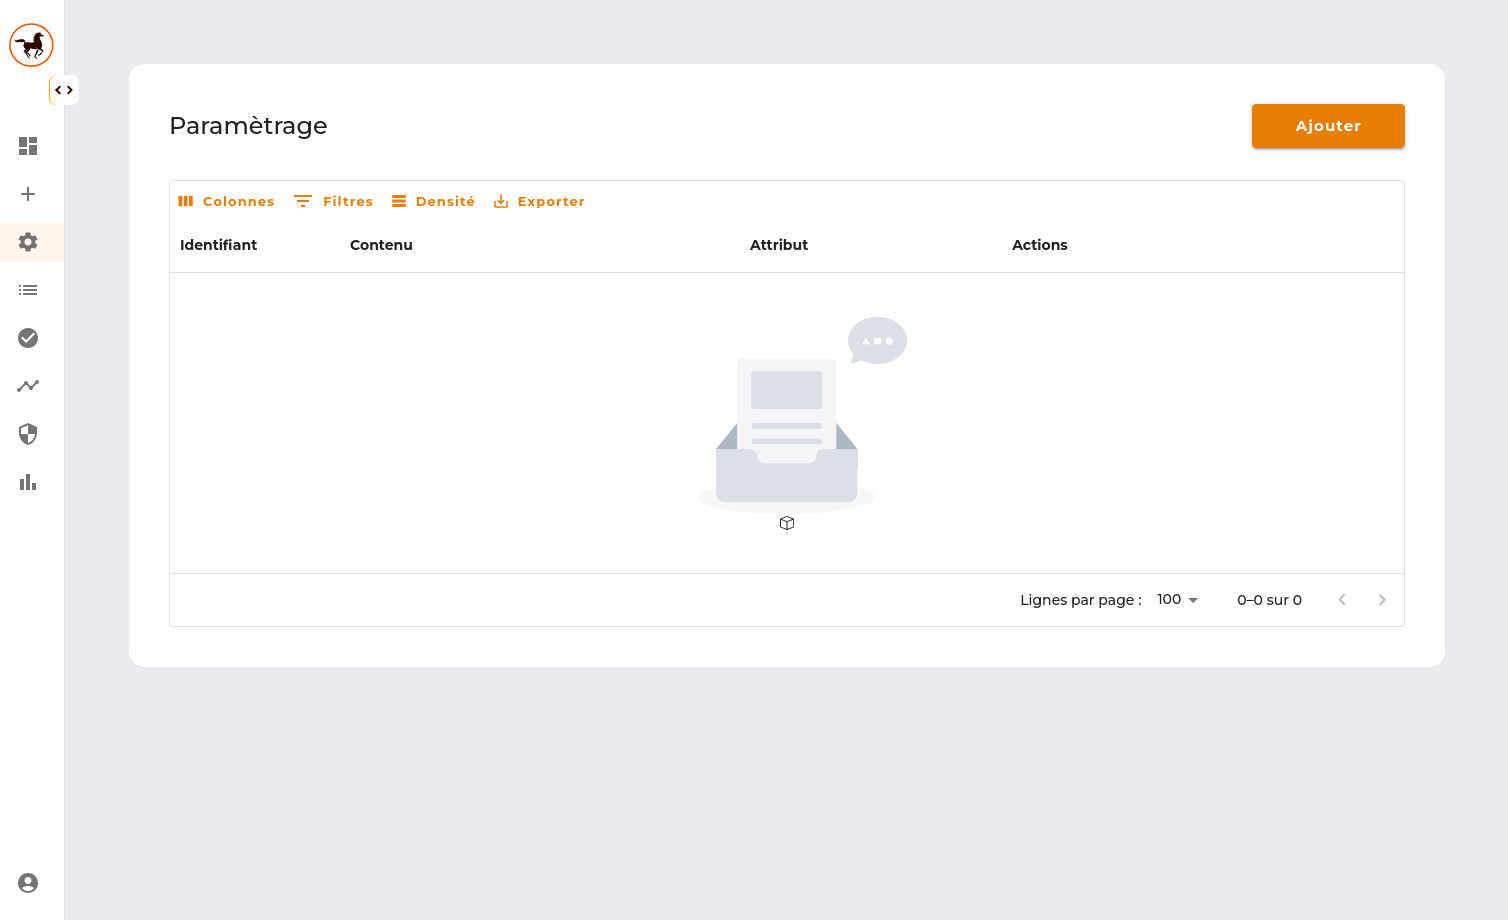
\includegraphics[width=\textwidth]{images/parametrage.png}
    \caption{Page de paramétrage}
\end{figure}

\clearpage


\subsection{Ajout d'une fiche de traitement}

\begin{figure}[H]
    \centering
    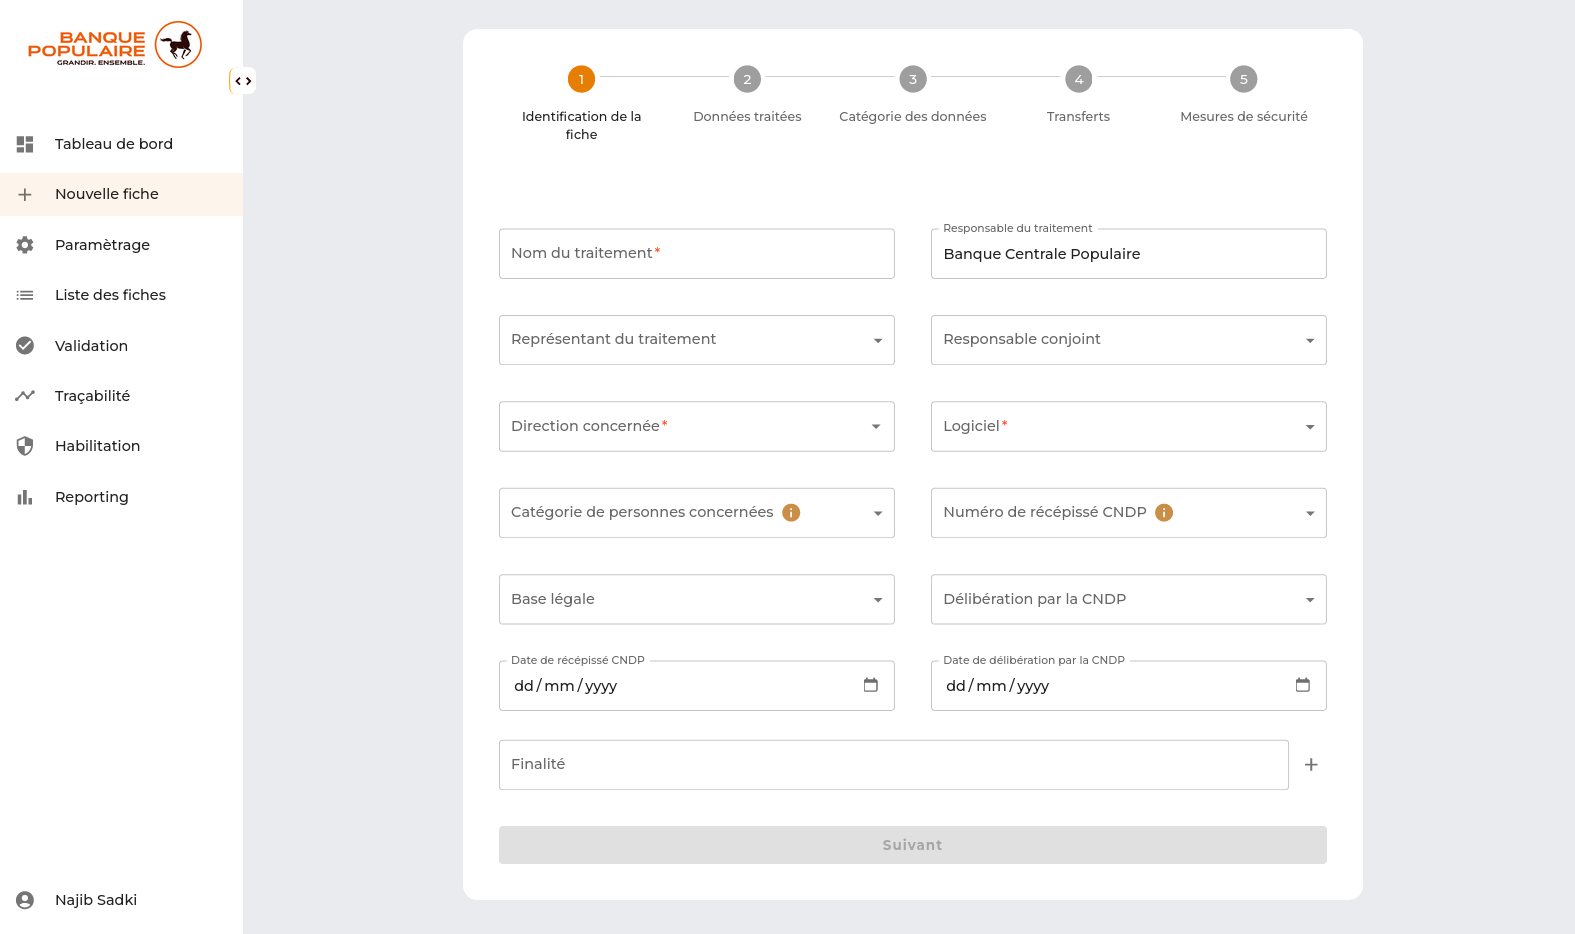
\includegraphics[width=\textwidth]{images/formulaire-fiche.png}
    \caption{Page d'ajout d'une fiche de traitement}
\end{figure}

\clearpage


\subsection{Liste des fiches de traitement}

\begin{figure}[H]
    \centering
    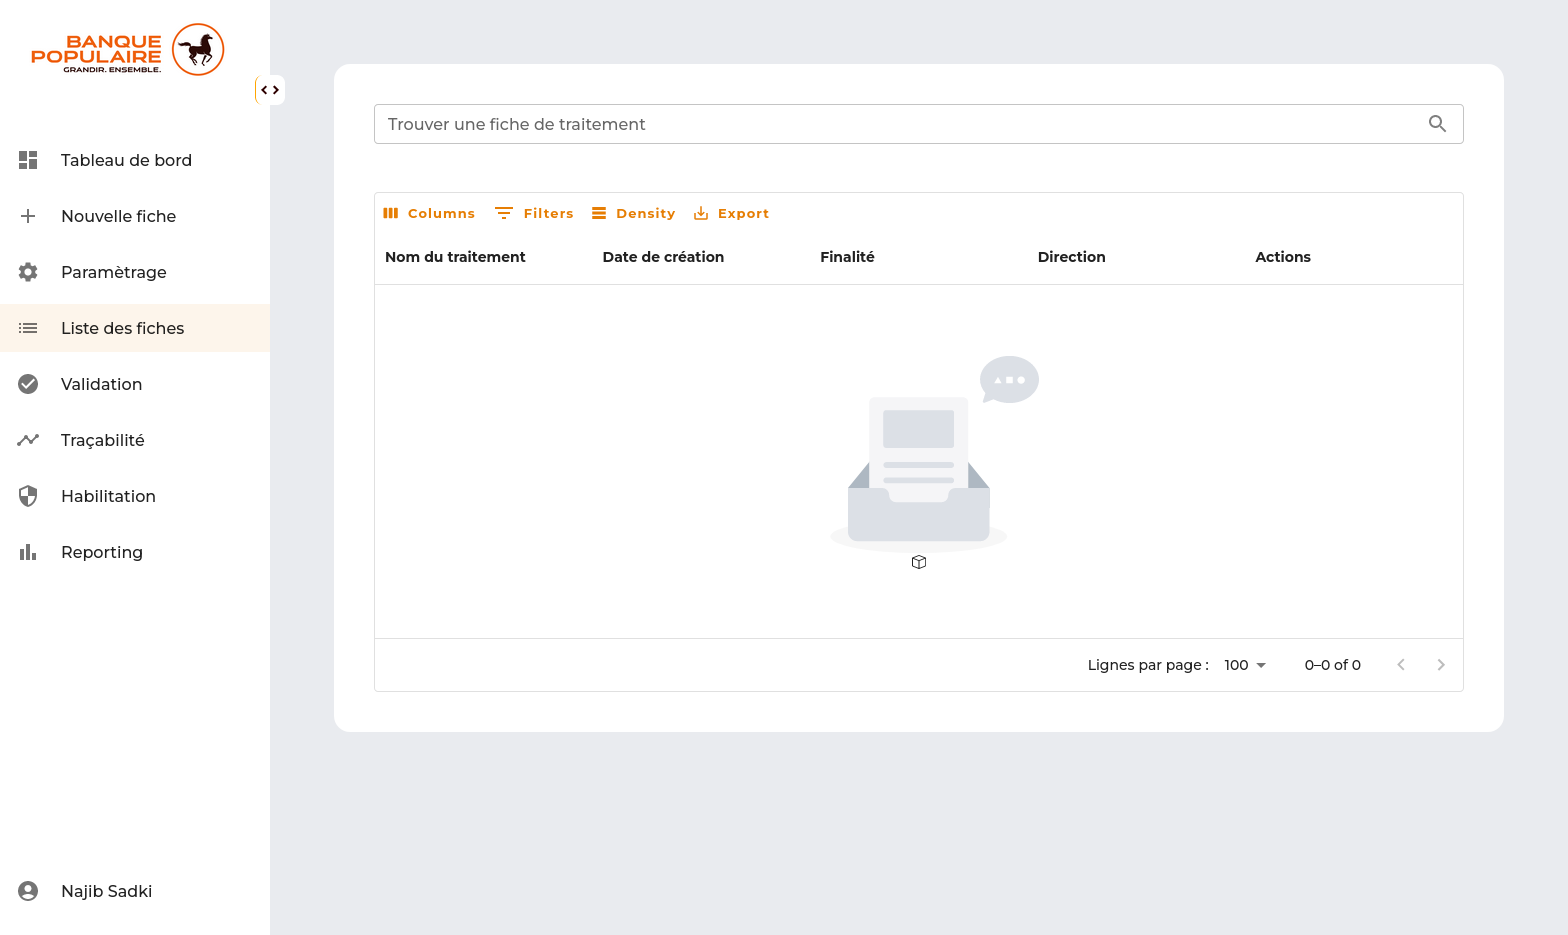
\includegraphics[width=1.35\textwidth, angle=90]{images/fiches.png}
    \caption{Page de la liste des fiches de traitement}
\end{figure}

\clearpage






